% Modelo relacional generado desde el esquema real con Anexos/Imagenes/fuentes/generar_modelo_relacional.py (17-oct-2026).
\section*{Modelo relacional} \label{modER}
\addcontentsline{toc}{section}{Modelo relacional}

La Figura \ref{fig:modeloER} muestra las tablas del dominio de Pymetory y sus llaves foráneas, tal como quedan definidas por las migraciones de Laravel. El anteproyecto lo llamaba modelo entidad-relación; como usa tablas y llaves, y no la notación de entidades y rombos, es un modelo relacional. Se omiten las tablas de infraestructura del framework (caché, colas, sesiones) y las de configuración sin relaciones (\texttt{settings}, \texttt{api\_keys}, \texttt{llm\_providers}, \texttt{custom\_field\_definitions}). La tabla \texttt{movimientos}, que implementa el Kardex, aparece resaltada; sus llaves hacia \texttt{lotes} y \texttt{users} impiden borrar un lote o un usuario que tenga historial.

\begin{figure}[H]
	\centering
	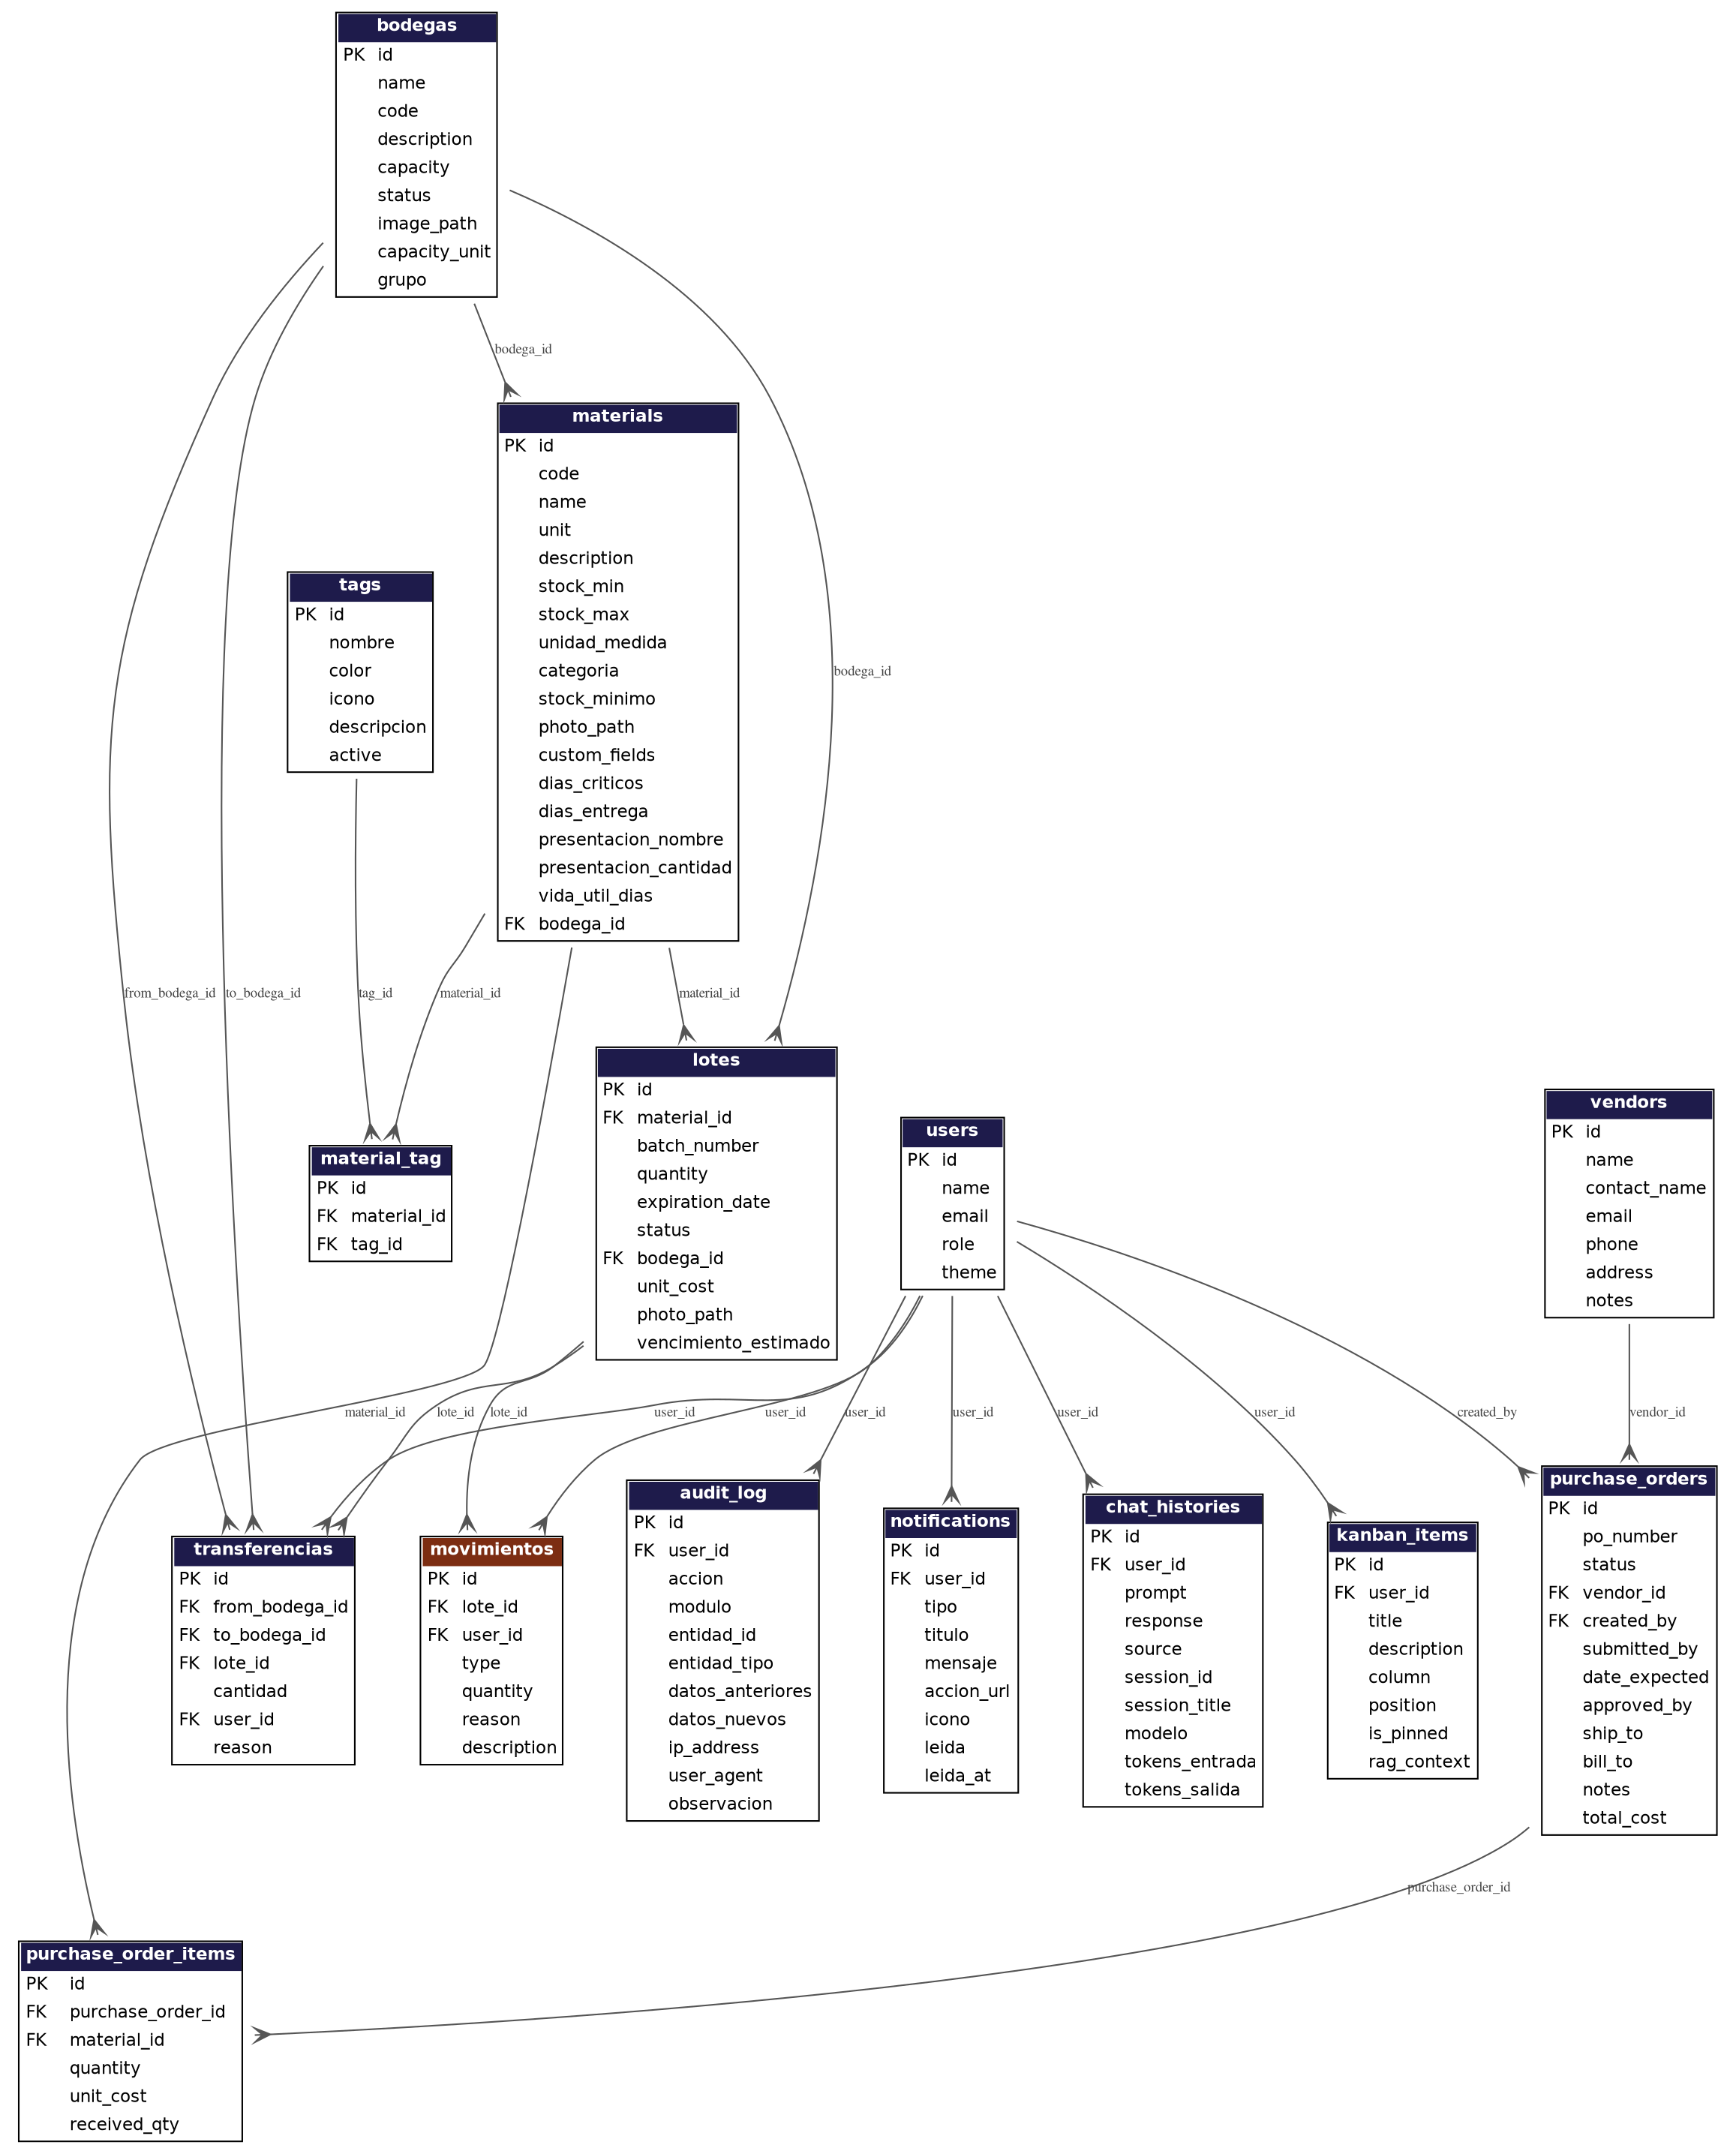
\includegraphics[width=0.9\textwidth]{Anexos/Imagenes/ModeloER_Pymetory.png}
	\caption{Modelo relacional de Pymetory.}
	\label{fig:modeloER}
\end{figure}
